\documentclass[../entwurf.tex]{subfiles}

\begin{document}

\section{ViewModel}
\subsection{AddSongPageVM}
\begin{minipage}{0.45\textwidth}
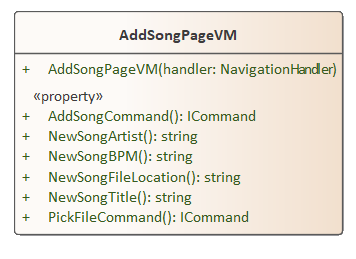
\includegraphics[scale=0.75]{../graphics/vm_klassen/AddSongPageVM.png}
\end{minipage}
\begin{minipage}{0.55\textwidth}
Diese Klasse enthält die UI-Logik der \code{AddSongsPage}. Sie stellt dieser öffentliche Eigenschaften und Commands zur Verfügung, welche dort an Steuerelemente gebunden sind, um als Bindeglied zwischen der \code{AddSongsPage} und dem Model zu dienen.
\end{minipage}
\paragraph{Attribute \& Properties}
\begin{itemize}
	\i{public string NewSongTitle} Hier wird der vom Nutzer eingegebene Titel eines neu hinzugefügten Lieds gespeichert.
	\i{public string NewSongArtist} Hier wird der vom Nutzer eingegebene Künstlername eines neu hinzugefügten Lieds gespeichert.
	\i{public string NewSongBPM} Hier wird der vom Nutzer eingegebene BPM-Wert eines neu hinzugefügten Lieds gespeichert.
	\i{public string NewSongFileLocation} Hier wird der vom Nutzer spezifizierte Pfad eines neu hinzugefügten Lieds gespeichert.
	\i{public ICommand\footnote{Stammt aus System.Windows.Input} AddSongCommand} Dieser Command führt die private Methode \code{AddSong()} aus. \glsnote{ro}
	\i{public ICommand PickFileCommand} Dieser Command führt die private Methode \code{PickFile()} aus. \glsnote{ro}
\end{itemize}
\paragraph{Methoden}
\begin{itemize}
	\i{public AddSongPageVM(AppLogic appLogic)} Der Konstruktor der Klasse initialisiert die Objekte \code{\_applogic}, \code{AddSongCommand} und \code{PickFileCommand}.
\end{itemize}
\subsection{AudioLibPageVM}
\begin{minipage}{0.55\textwidth}
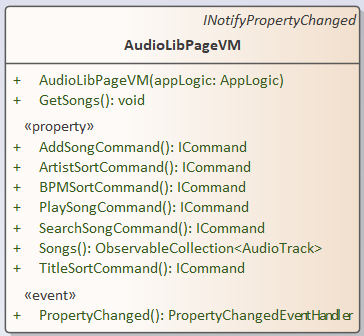
\includegraphics[scale=0.75]{../graphics/vm_klassen/AudioLibPageVM.png}
\end{minipage}
\begin{minipage}{0.45\textwidth}
Diese Klasse enthält die UI-Logik der \code{AudioLibPage}. Sie stellt dieser öffentliche Eigenschaften und Commands zur Verfügung, welche dort an Steuerelemente gebunden sind, um als Bindeglied zwischen der \code{AudioLibPage} und dem Model zu dienen.
\end{minipage}
\paragraph{Attribute \& Properties}
\begin{itemize}
	\i{public ObservableCollection<AudioTrack> Songs} Hier werden die Songs gespeichert, die in der View angezeigt werden sollen.
	\i{public ICommand TitleSortCommand} Dieser Command führt die private Methode \code{TitleSort()} aus. \glsnote{ro}
	\i{public ICommand ArtistSortCommand} Dieser Command führt die private Methode \code{ArtistSort()} aus. \glsnote{ro}
	\i{public ICommand BPMSortCommand} Dieser Command führt die private Methode \code{BPMSort()} aus. \glsnote{ro}
	\i{public ICommand PlaySongCommand} Dieser Command führt die private Methode \code{PlaySong()} mit dem in der View ausgewählten Song als Parameter aus. \glsnote{ro}
	\i{public ICommand AddSongCommand} Dieser Command führt die private Methode \code{AddSong()} aus. \glsnote{ro}
	\i{public ICommand SearchSongCommand} Dieser Command führt die private Methode \code{SearchSong()} mit dem in der View eingegeben Text als Parameter aus. \glsnote{ro}
\end{itemize}
\paragraph{Methoden}
\begin{itemize}
	\i{public AudioLibPageVM(AppLogic appLogic)} Der Konstruktor der Klasse initialisiert die Objekte \code{\_applogic}, \code{Songs} und die Commands.
	\i{public void GetSongs()} Diese Methode ruft die Songs ab, die im Model gespeichert sind und weist sie der Property \code{Songs} zu.
	\i{public event PropertyChangedEventHandler PropertyChanged} Dieses Event wird genutzt um der View mitzuteilen, dass sich eine Property geändert hat.
\end{itemize}
\subsection{AudioPlayerPageVM}
\begin{minipage}{0.55\textwidth}
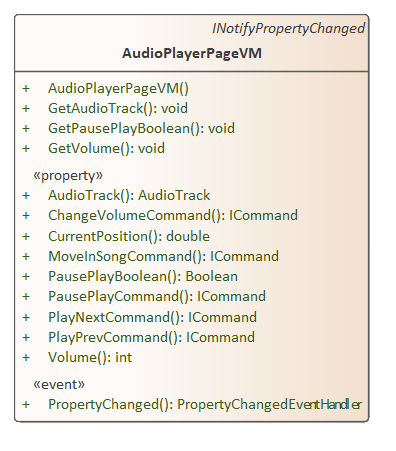
\includegraphics[scale=0.75]{../graphics/vm_klassen/AudioPlayerPageVM.png}
\end{minipage}
\begin{minipage}{0.45\textwidth}
Diese Klasse enthält die UI-Logik der \code{AudioPlayerPage}. Sie stellt dieser öffentliche Eigenschaften und Commands zur Verfügung, welche dort an Steuerelemente gebunden sind, um als Bindeglied zwischen der \code{AudioPlayerPage} und dem Model zu dienen.
\end{minipage}
\paragraph{Attribute \& Properties}
\begin{itemize}
	\i{public Boolean PausePlayBoolean} Dieser Boolean gibt an, ob der AudioPlayer momentan aktiv oder pausiert ist.
	\i{public AudioTrack AudioTrack} Hier wird der momentan im Model geladene Song gespeichert.
	\i{public int Volume} Hier wird der Wert der Lautstärke gespeichert.
	\i{public double CurrentPosition} Hier wird die aktuelle Position im momentan aktiven Song gespeichert.
	\i{public Image Icon} Je nachdem ob der AudioPlayer aktiv oder pausiert ist, ist hier ein bestimmtes Bild gespeichert.
	\i{public ICommand PausePlayCommand} Dieser Command führt die private Methode \code{PausePlay()} aus. \glsnote{ro}
	\i{public ICommand PlayPrevCommand} Dieser Command führt die private Methode \code{PlayPrev()} aus. \glsnote{ro}
	\i{public ICommand PlayNextCommand} Dieser Command führt die private Methode \code{PlayNext()} aus. \glsnote{ro}
	\i{public ICommand ChangeVolumeCommand} Dieser Command führt die private Methode \code{ChangeVolume()} mit der in der View ausgewählten Lautstärke als Parameter aus.
	\i{public ICommand MoveInSongCommand} Dieser Command führt die private Methode \code{MoveInSong()} mit der in der View ausgewählten Position als Parameter aus.
\end{itemize}
\paragraph{Methoden}
\begin{itemize}
	\i{public AudioPlayerPageVM(AppLogic appLogic)} Der Konstruktor der Klasse initialisiert die Objekte \code{\_applogic}, die Icons und die Commands.
	\i{public void GetAudioTrack()} Diese Methode ruft den im Model momentan geladenen Song ab und weist sie der Property \code{Songs} zu.
	\i{public void GetPausePlayBoolean()} Diese Methode ruft im Model ab, ob der Audioplayer aktiv oder pausiert werden soll und weist den Boolean der Property \code{PausePlayBoolean} zu.
	\i{public void GetVolume()} Diese Methode ruft im Model ab, ob der Audioplayer aktiv oder pausiert werden soll und weist den Boolean der Property \code{PausePlayBoolean} zu.
	\i{public event PropertyChangedEventHandler PropertyChanged} Dieses Event wird genutzt um der View mitzuteilen, dass sich eine Property geändert hat.
\end{itemize}
\subsection{ConnectionPageVM}
\begin{minipage}{0.55\textwidth}
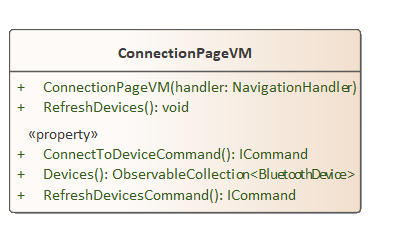
\includegraphics[scale=0.75]{../graphics/vm_klassen/ConnectionPageVM.png}
\end{minipage}
\begin{minipage}{0.45\textwidth}
Diese Klasse enthält die UI-Logik der \code{ConnectionPage}. Sie stellt dieser öffentliche Eigenschaften und Commands zur Verfügung, welche dort an Steuerelemente gebunden sind, um als Bindeglied zwischen der \code{ConnectionPage} und dem Model zu dienen.
\end{minipage}
\paragraph{Attribute \& Properties}
\begin{itemize}
	\i{public ObservableCollection<IEarable> Devices} Hier werden die Geräte gepeichert die in der View angezeigt werden sollen.
	\i{public ICommand RefreshDevicesCommand} Dieser Command führt die private Methode \code{RefreshDevices()} aus. \glsnote{ro}
	\i{public ICommand ConnectToDeviceCommand} Dieser Command führt die private Methode \code{ConnectToDevice()} mit dem in der View ausgewähltem Gerät als Parameter aus. \glsnote{ro}
\end{itemize}
\paragraph{Methoden}
\begin{itemize}
	\i{public ConnectionPageVM(AppLogic appLogic)} Der Konstruktor der Klasse initialisiert die Objekte \code{\_applogic}, \code{Devices} und die Commands.
	\i{public void RefreshDevices()} Diese Methode ruft den im Model momentan erkannten Geräte ab und fügt sie der Property \code{Devices} hinzu.
	\i{public event PropertyChangedEventHandler PropertyChanged} Dieses Event wird genutzt um der View mitzuteilen, dass sich eine Property geändert hat.
\end{itemize}
\subsection{MainPageVM}
\begin{minipage}{0.55\textwidth}
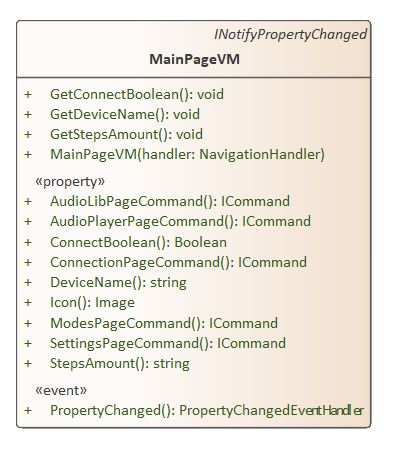
\includegraphics[scale=0.75]{../graphics/vm_klassen/MainPageVM.png}
\end{minipage}
\begin{minipage}{0.45\textwidth}
Diese Klasse enthält die UI-Logik der \code{MainPage}. Sie stellt dieser öffentliche Eigenschaften und Commands zur Verfügung, welche dort an Steuerelemente gebunden sind, um als Bindeglied zwischen der \code{MainPage} und dem Model zu dienen.
\end{minipage}
\paragraph{Attribute \& Properties}
\begin{itemize}
	\i{public string DeviceName} Hier wird der Name des momentan verbundenen Geräts gespeichert, falls keine Verbindung besteht, hat der String den wert null.
	\i{public string StepsAmount} Hier wird die Anzahl der Schritte seit dem letzten Reset gespeichert, falls keine Verbindung zu einem Gerät besteht, hat der String den wert null.
	\i{public Boolean ConnectBoolean} Dieser Boolean gibt an, ob eine Verbindung zu einem Gerät besteht.
	\i{public Image Icon} Je nachdem ob eine Verbindung zu einem Gerät besteht oder nicht, ist hier ein bestimmtes Bild gespeichert.
	\i{public ICommand AudioPlayerPageCommand} Dieser Command führt die private Methode \code{GotoAudioPlayerPage()} aus. \glsnote{ro}
	\i{public ICommand AudioLibPageCommand} Dieser Command führt die private Methode \code{GotoAudioLibPage()} aus. \glsnote{ro}
	\i{public ICommand ConnectionPageCommand} Dieser Command führt die private Methode \code{GotoConnectionPage()} aus. \glsnote{ro}
	\i{public ICommand ModesPageCommand} Dieser Command führt die private Methode \code{GotoModesPage()} aus. \glsnote{ro}
	\i{public ICommand SettingsPageCommand} Dieser Command führt die private Methode \code{GotoSettingsPage()} aus. \glsnote{ro}
\end{itemize}
\paragraph{Methoden}
\begin{itemize}
	\i{public MainPageVM(AppLogic appLogic)} Der Konstruktor der Klasse initialisiert die Objekte \code{\_applogic}, die Icons und die Commands.
	\i{public void GetDeviceName()} Diese Methode ruft den Namen des momentan verbundenen Gerätes ab und weist sie der Property \code{DeviceName} zu.
	\i{public void GetStepsAmount()} Diese Methode ruft im Model ab, wie viele Schritte seit dem letztem Reset gemacht wurden und weist den Wert der Property \code{StepsAmount} zu.
	\i{public void GetConnectBoolean()} Diese Methode ruft im Model ab, ob momentan eine Verbindung zu einem Gerät besteht und weist den Boolean der Property \code{ConnectBoolean} zu.
	\i{public event PropertyChangedEventHandler PropertyChanged} Dieses Event wird genutzt um der View mitzuteilen, dass sich eine Property geändert hat.
\end{itemize}
\subsection{ModesPageVM}
\begin{minipage}{0.55\textwidth}
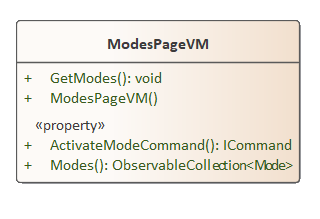
\includegraphics[scale=0.75]{../graphics/vm_klassen/ModesPageVM.png}
\end{minipage}
\begin{minipage}{0.45\textwidth}
Diese Klasse enthält die UI-Logik der \code{ModesPage}. Sie stellt dieser öffentliche Eigenschaften und Commands zur Verfügung, welche dort an Steuerelemente gebunden sind, um als Bindeglied zwischen der \code{ModesPage} und dem Model zu dienen.
\end{minipage}
\paragraph{Attribute \& Properties}
\begin{itemize}
	\i{public ObservableCollection<Mode> Modes} Hier werden die Modi gespeichert, die in der View angezeigt werden sollen.
	\i{public ICommand ActivateModeCommand} Dieser Command führt die private Methode \code{ActivateMode()} mit dem in der View ausgewählten Modus als Parameter aus. \glsnote{ro}
\end{itemize}
\paragraph{Methoden}
\begin{itemize}
	\i{public ModesPageVM(AppLogic appLogic)} Der Konstruktor der Klasse initialisiert die Objekte \code{\_applogic} und die Commands.
	\i{public void GetModes()} Diese Methode ruft die im Model vorhandenen Modi ab und weist sie der Property \code{Modes} zu.
	\i{public event PropertyChangedEventHandler PropertyChanged} Dieses Event wird genutzt um der View mitzuteilen, dass sich eine Property geändert hat.
\end{itemize}
\subsection{SettingsPageVM}
\begin{minipage}{0.55\textwidth}
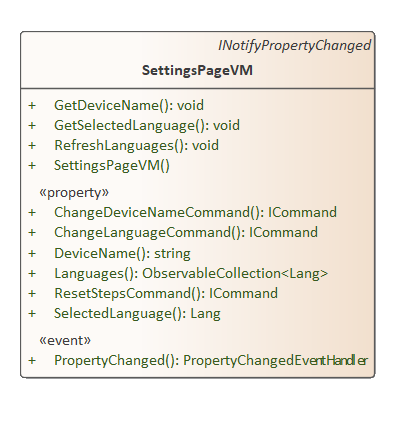
\includegraphics[scale=0.75]{../graphics/vm_klassen/SettingsPageVM.png}
\end{minipage}
\begin{minipage}{0.45\textwidth}
Diese Klasse enthält die UI-Logik der \code{SettingsPage}. Sie stellt dieser öffentliche Eigenschaften und Commands zur Verfügung, welche dort an Steuerelemente gebunden sind, um als Bindeglied zwischen der \code{SettingsPage} und dem Model zu dienen.
\end{minipage}
\paragraph{Attribute \& Properties}
\begin{itemize} 
	\i{public ObservableCollection<Lang> Languages} Hier werden die Sprachen gespeichert, die in der View angezeigt werden sollen.
	\i{public Lang SelectedLanguage} Hier wird die Sprache gespeichert, die in der View als ausgewählt angezeigt wird.
	\i{public string DeviceName} Hier wird der Name des momentan verbundenen Geräts gepeichert der in der View angezeigt wird.
	\i{public ICommand ChangeDeviceNameCommand} Dieser Command führt die private Methode \code{ChangeDeviceName()} mit dem in der View eingegebenen Text als Parameter aus. \glsnote{ro}
	\i{public ICommand ChangeLanguageCommand} Dieser Command führt die private Methode \code{ChangeLanguage()} mit der in der View ausgewählten Sprache als Parameter aus. \glsnote{ro}
	\i{public ICommand ResetStepsCommand} Dieser Command führt die private Methode \code{ResetSteps()} aus. \glsnote{ro}
\end{itemize}
\paragraph{Methoden}
\begin{itemize}
	\i{public SettingsPageVM(AppLogic appLogic)} Der Konstruktor der Klasse initialisiert die Objekte \code{\_applogic} und die Commands.
	\i{public void RefreshLanguages()} Diese Methode ruft die im Model vorhandenen Sprachen ab und weist sie der Property \code{Languages} zu.
	\i{public void GetSelectedLanguage()} Diese Methode ruft die im Model ausgewählte Sprache ab und weist sie der Property \code{SelectedLanguage} zu.
	\i{public void GetDeviceName()} Diese Methode ruft den Namen des momentan verbundenen Gerätes im Model ab und weist ihn der Property \code{DeviceName} zu.
	\i{public event PropertyChangedEventHandler PropertyChanged} Dieses Event wird genutzt um der View mitzuteilen, dass sich eine Property geändert hat.
\end{itemize}
\subsection{NavigationHandler}
\paragraph{Attribute \& Properties}
\paragraph{Methoden}
\begin{itemize}
	\i{public SettingsPageVM(AppLogic appLogic)} Der Konstruktor der Klasse initialisiert alle Attribute.
	\i{public static async void GotoPage()} TODO
	\i{public static async void GoBack()} Diese Methode ändert die Ansicht der View auf die Page die zuvor angezeigt wurde
\end{itemize}

\end{document}
